\documentclass{beamer}
%\usepackage{fontspec}

\usetheme{Boadilla}
%\setmainfont{Latin Modern Sans}

%\includeonlyframes{current}

\usefonttheme{structurebold}
\usepackage{listings}
\usepackage{ragged2e}

\usepackage{pgf}
\usepackage{tikz}
\usepackage{alltt}
\usepackage[normalem]{ulem}
\usetikzlibrary{arrows}
\usetikzlibrary{automata}
\usetikzlibrary{shapes}
\usepackage{amsmath,amssymb}
\usepackage{rotating}
\usepackage{ulem}
\usepackage{listings}
\usepackage{enumerate}
\usepackage{tikz}
\tikzset{
  every overlay node/.style={
    draw=black,fill=white,rounded corners,anchor=north west,
  },
}
\def\tikzoverlay{%
   \tikz[baseline,overlay]\node[every overlay node]
}%

%\setbeamercovered{dynamic}
\setbeamertemplate{footline}[page number]{}
\setbeamertemplate{navigation symbols}{}
\usefonttheme{structurebold}

\title{Software Testing, Quality Assurance \& Maintenance---Lecture 26}
\author{Patrick Lam}
\date{March 10, 2017}

\colorlet{redshaded}{red!25!bg}
\colorlet{shaded}{black!25!bg}
\colorlet{shadedshaded}{black!10!bg}
\colorlet{blackshaded}{black!40!bg}

\colorlet{darkred}{red!80!black}
\colorlet{darkblue}{blue!80!black}
\colorlet{darkgreen}{green!80!black}

\newcommand{\rot}[1]{\rotatebox{90}{\mbox{#1}}}
\newcommand{\gray}[1]{\mbox{#1}}

\newenvironment{changemargin}[1]{% 
  \begin{list}{}{% 
    \setlength{\topsep}{0pt}% 
    \setlength{\leftmargin}{#1}% 
    \setlength{\rightmargin}{1em}
    \setlength{\listparindent}{\parindent}% 
    \setlength{\itemindent}{\parindent}% 
    \setlength{\parsep}{\parskip}% 
  }% 
  \item[]}{\end{list}}


\lstset{ %
language=C++,
basicstyle=\ttfamily,commentstyle=\scriptsize\itshape,showstringspaces=false,breaklines=true}

\begin{document}

\begin{frame}
  \titlepage
\end{frame}

\begin{frame}
\frametitle{Last Time}
  \Large
  \begin{changemargin}{1cm}
    Practical techniques for writing tests.\\[1em]

    Result verification:
    \begin{itemize}
    \item state verification;
    \item behaviour verification.
    \end{itemize}~\\

    Also, techniques for improving your tests.
    \begin{itemize}
    \item reducing duplication
    \item simplifying tests
    \end{itemize}

  \end{changemargin}
\end{frame}

\begin{frame}
  \frametitle{Today: More Test Design}

  \Large
  \begin{changemargin}{2cm}
\begin{itemize}
\item Mock objects;
\item Flaky tests;
\item Continuous integration;
%\item Hermetic tests.
\end{itemize}
  \end{changemargin}

\end{frame}

\begin{frame}
  \frametitle{Mock Objects}
  \begin{center}
    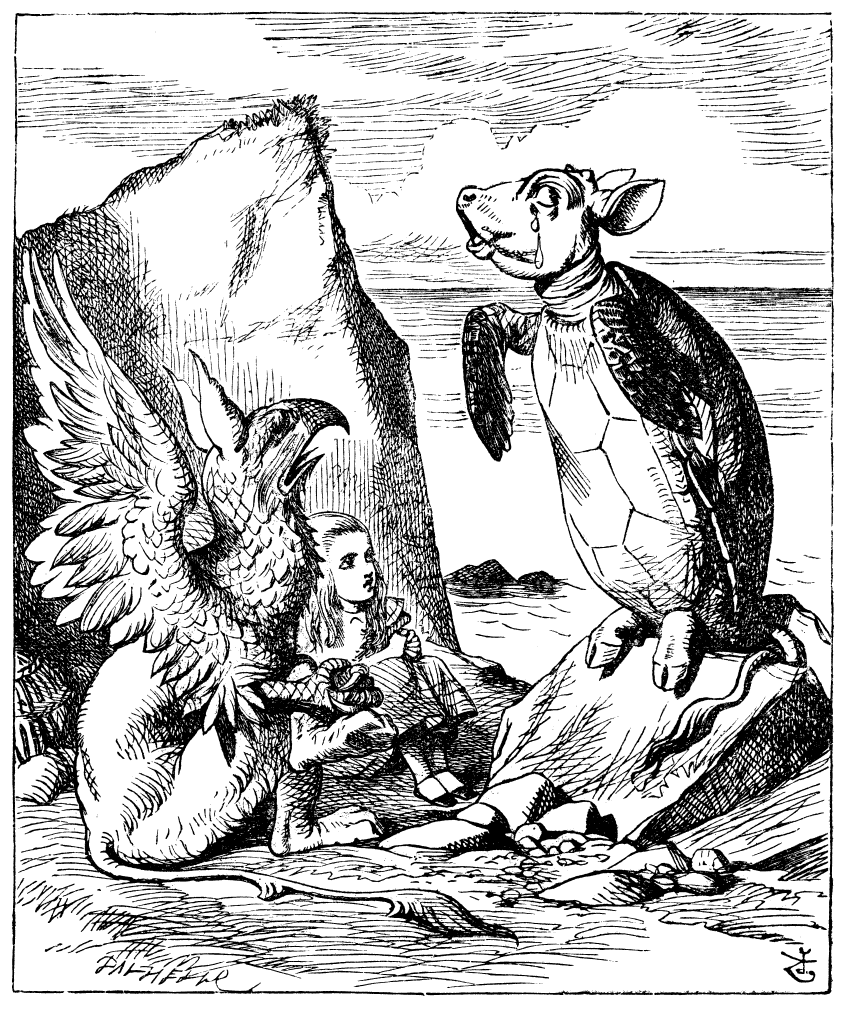
\includegraphics[height=.8\textheight]{L26/Alice_par_John_Tenniel_34.png}\\
John Tenniel's original (1865) illustration for Lewis Carroll's ``Alice in Wonderland''. Alice sitting between Gryphon and Mock turtle.
  \end{center}
\end{frame}

\begin{frame}
  \frametitle{Test Doubles}
  \begin{changemargin}{1cm}
    Meszaros proposes four kinds of test doubles:
    \begin{itemize}
    \item dummy objects (don't do anything);
    \item fake objects (do something, but no good in prod, \\ \hspace*{3cm} e.g. in-memory database);
    \item stubs (canned answers)
    \item spies (stubs/proxies that record interactions);
      \item mocks (objects with expectations)
    \end{itemize}
    Reference: \\ \url{martinfowler.com/articles/mocksArentStubs.html}
\end{changemargin}
\end{frame}

\begin{frame}[fragile]
  \frametitle{Mail Service Stub}
{\small    \begin{lstlisting}
public class MailServiceStub implements MailService {
  private List<Message> messages =
     new ArrayList<Message>();
  public void send (Message msg) {
    messages.add(msg);
  }
  public int numberSent() {
    return messages.size();
  }
}     
  \end{lstlisting}
  }
    \begin{changemargin}{1cm}
      good for state verification:
\begin{lstlisting}      
  assertEquals(1, mailer.numberSent());
\end{lstlisting}
    \end{changemargin}
\end{frame}

\begin{frame}[fragile]
  \frametitle{Using Mocks}
{\small    \begin{lstlisting}
class OrderInteractionTester...

  public void testOrderSendsMailIfUnfilled() {
    Order order = new Order(TALISKER, 51);
    Mock warehouse = mock(Warehouse.class);
    Mock mailer = mock(MailService.class);
    order.setMailer((MailService) mailer.proxy());

    mailer.expects(once()).method("send");
    warehouse.expects(once()).method("hasInventory")
      .withAnyArguments()
      .will(returnValue(false));

    order.fill((Warehouse) warehouse.proxy());
  }
}
  \end{lstlisting}}
\end{frame}

\begin{frame}[fragile]
  \frametitle{Creating Mock Objects with EasyMock\footnote{http://easymock.org/user-guide.html}}
%import static org.easymock.EasyMock.*;
%import org.easymock.EasyMockRunner;
%import org.easymock.TestSubject;
%import org.easymock.Mock;
%import org.junit.Test;
%import org.junit.runner.RunWith;

  {\small \begin{lstlisting}
@RunWith(EasyMockRunner.class)
public class ExampleTest {

  @TestSubject
  private ClassUnderTest classUnderTest = new ClassUnderTest();

  @Mock // creates a mock object
  private Collaborator mock;

  @Test
  public void testRemoveNonExistingDocument() {
    replay(mock);
    classUnderTest.removeDocument("Does not exist");
  }
}      
               \end{lstlisting}
               }
\end{frame}

\begin{frame}[fragile]
  \frametitle{Expecting behaviour: method calls}
{\small
  \begin{lstlisting}
@Test
public void testAddDocument() {
  // recording phase:
  mock.documentAdded("New Document");
  replay(mock);
  // replaying phase; we expect the recorded actions to happen
  classUnderTest.addDocument("New Document",
                             new byte[0]);
  // check that the behaviour actually happened:
  verify(mock);
}
  \end{lstlisting}
  }
\end{frame}

\begin{frame}[fragile]
  \frametitle{Expecting behaviour: return values}
{\small
  \begin{lstlisting}
@Test
public void testVoteForRemoval() {
  // expect document addition
  mock.documentAdded("Document");
  // expect to be asked to vote for document removal, and vote for it
  expect(mock.voteForRemoval("Document"))
             .andReturn((byte) 42);
  // expect document removal
  mock.documentRemoved("Document");
  replay(mock);
  classUnderTest.addDocument("Document", new byte[0]);
  assertTrue
    (classUnderTest.removeDocument("Document"));
  verify(mock);
}  \end{lstlisting}
  }
\end{frame}

% http://www.tutorialspoint.com/easymock/easymock_adding_behavior.htm

\begin{frame}
  \frametitle{Flakiness: Good for croissants\footnote{thanks Pixabay}, bad for tests}
  
\includegraphics[width=\textwidth]{L26/croissant-410322_1920.jpg}
\end{frame}

\begin{frame}
  \frametitle{Reference}

  \begin{changemargin}{1cm}
    Qingzhou Luo, Farah Hariri, Lamyaa Eloussi, Darko Marinov. ``An Empirical Analysis of Flaky Tests''. In FSE '14.
  \end{changemargin}
\end{frame}

\begin{frame}
  \frametitle{What Are Flaky Tests?}
  \begin{changemargin}{1cm}
    \Large
    Flaky test = sometimes fails (nondeterministically).
  \end{changemargin}
\end{frame}

\begin{frame}
  \frametitle{Dealing with Flaky Tests}
  \begin{changemargin}{1cm}
    \Large
    \begin{itemize}
    \item Label as flaky.
    \item Re-run tests, see if it ever passes.
    \item Ignore/remove flaky tests.
    \end{itemize}
  \end{changemargin}
\end{frame}

\begin{frame}
  \frametitle{What causes flakiness?}
  \Large
  \begin{changemargin}{1cm}
    Result of studying 201 fixes:
    \begin{itemize}
    \item improper wait for async responses;
    \item concurrency;
    \item test order dependency;
    \item etc.
    \end{itemize}
  \end{changemargin}
\end{frame}

\begin{frame}
  \frametitle{Async Wait}
  \Large
  \begin{changemargin}{.6cm}
    Problem: \\
    \hspace*{1cm} do something, then sleep for not-long enough.\\
    Solution: \\
    \hspace*{1cm} use a {\tt wait} call to wait until the thing happens.
  \end{changemargin}
\end{frame}

\begin{frame}
  \frametitle{Concurrency}
  \Large
  \begin{changemargin}{1cm}
    Usual concurrency problems:
    \begin{itemize}
    \item data races;
    \item atomicity violations;
    \item deadlocks.
    \end{itemize}
    May be in test or the system under test.
  \end{changemargin}
\end{frame}

\begin{frame}
  \frametitle{Test Order Dependency}
  \Large
  \begin{changemargin}{1cm}
    Problem: test X expects test Y to have completed.\\
    Solution: remove dependency.
  \end{changemargin}
\end{frame}

\begin{frame}
  \frametitle{Continuous Integration}

  \Large
  \begin{changemargin}{2cm}
    Literally:
  \end{changemargin}
    \begin{center}
      use a single shared master branch
    \end{center}
\end{frame}

\begin{frame}
  \frametitle{Why This Is Continuous Integration}

  \Large
  \begin{changemargin}{2cm}
    \begin{tabbing}
    Integration = \= merge one's changes \\
    \> back into master.
    \end{tabbing}
    ~\\
    Continuous = do it all the time.
  \end{changemargin}
\end{frame}

\begin{frame}
  \frametitle{Why CI Is Awesome}

  \Large
  \begin{changemargin}{1cm}
    Software stays in working state.\\[1em]
    Developers don't integrate for months-on-end.
  \end{changemargin}
\end{frame}

\begin{frame}
  \frametitle{Things that go with CI}

  \Large
  \begin{changemargin}{1cm}
    Continuous Builds\\[1em]
    Test Automation\\[1em]
    Continuous Deployment (optional)
  \end{changemargin}
\end{frame}

\begin{frame}
  \frametitle{What Happens In CI}

  \Large
  \begin{changemargin}{1cm}
    \begin{enumerate}
    \item You clone the repo (which works).
    \item You make your changes.
    \item You commit and push your changes (often!)
    \item A machine pulls the changes, compiles them, and runs automated tests.
      \item Everyone knows whether your changes passed tests or not.
    \end{enumerate}
  \end{changemargin}
\end{frame}

\begin{frame}
  \frametitle{Continuous Deployment}

  \Large
  \begin{changemargin}{1cm}
    Minor variation to CI: \\
    \begin{changemargin}{1cm}
      production machine also pulls changes as soon as tests pass.
    \end{changemargin}
  \end{changemargin}
\end{frame}

\begin{frame}
  \frametitle{Key Details}

  \Large
  \begin{changemargin}{1cm}
    \begin{itemize}
    \item Fix broken builds immediately!
    \item Keep the build fast (minutes):\\
      \hspace*{1cm} parallelize it \& tier your tests.
    \item Test in a prod-like environment.
    \end{itemize}
      
  \end{changemargin}
\end{frame}


\begin{frame}
  \frametitle{Continuous Integration References}

  \begin{changemargin}{1cm}
    Bullet points from Gitlab: \\
    \url{about.gitlab.com/2015/02/03/7-reasons-why-you-should-be-using-ci/}\\[1em]
    Mid-length article from Atlassian: \\
\url{www.atlassian.com/agile/continuous-integration}\\[1em]
    Longer article by Martin Fowler: \\
    \url{martinfowler.com/articles/continuousIntegration.html}\\[2em]
    Serverless CI: \\
    \url{medium.com/@hichaelmart/lambci-4c3e29d6599b}
  \end{changemargin}
\end{frame}



\begin{frame}
  \frametitle{Summary}
  \Large
  \begin{changemargin}{1cm}
    More practical techniques for writing tests:\\[1em]

    How to actually do behaviour verification (mock objects).\\
    Pitfalls of bad test writing (flaky tests).\\
    Making sure your code's always good (CI).\\
    %Running your tests without dependencies (hermetic tests).

  \end{changemargin}
\end{frame}


\end{document}
